\documentclass{TDP005mall}

\usepackage{mathtools}
\usepackage{float}

\newcommand{\version}{Version 0.1}
\author{David Dumminsek, \url{davdu153@student.liu.se}\\
  Haris Basic, \url{harba466@student.liu.se}\\}
\title{Designspecifikation}
\date{2022-11-24}
\rhead{David Dumminsek\\
Haris Basic\\}



\begin{document}
\projectpage
\section{Revisionshistorik}
\begin{table}[!h]
\begin{tabularx}{\linewidth}{|l|X|l|}
\hline
Ver. & Revisionsbeskrivning & Datum \\\hline
  0.1 & första utkast & 2022-11-24\\\hline
\end{tabularx}
\end{table}


\section{Klasser}
Vilka klassar som kommer användas i spelet.

\subsection{Player}
Denna klass ska modellera spelaren.
Det ska vara möjligt för spelaren att röra sig, kollidera och skjuta projektiler.
\subsubsection*{Klassrelationer}
\begin{enumerate}
  \item \textbf{Projectile:} Player använder ett projectile objekt för att beskriva hur Player projektilen fungerar.\\
                    Om player delar koordinater med en projektil så dör spelaren.
  \item \textbf{Enemy:} Om ett Player objekt delar koordinater med ett Enemy objekt dör spelaren.
  \item \textbf{Game:} Vart Player objektet skapas.
\end{enumerate}
\subsubsection*{Konstruktorer}
\begin{enumerate}
  \item \textbf{Player()} Sätter \textbf{life} till 2, \textbf{speed} till 0.1 och koordinaterna till det som är mitt i botten. Samt så konstrueras ett Projectile objekt.
  \item \textbf{Player(Projectile a):} Är lik default constructorn utom att en valfri Projecile objekt kan användas.
\end{enumerate}
\subsubsection*{Variabler}
\begin{enumerate}
  \item \textbf{int x{}:} x koordinater för spelaren
  \item \textbf{int y{}:} y koordinater för spelaren
  \item \textbf{float speed{}:} hur många x eller y koordinater spelaren rör sig per tick.
  %\item \textbf{int point:} hur många poäng spelaren har
  \item \textbf{int life{}:} hur många liv spelaren har.
  \item \textbf{Projectile pro{}:} Projectile object som beskriver hur projektilen rör sig och hur mycket skada den gör:'
\end{enumerate}
\subsubsection*{Funktioner}
\begin{enumerate}
  \item \textbf{void move():} Tar emot användarinmatning från game loopet och updaterar koordinaterna med \textbf{speed} variablen.
    Om koordinaterna skulle hamna utanför spelet så ändras inte koordinaterna (fiende kollidering kommer hanteras i \textbf{Game} klassen). 
  \item \textbf{void shoot():} Skapar \textbf{Projectile} objekt som startar med \textbf{Player} koordinaterna och rör sig rakt fram i en hastighet beroende på objektet. 
  \item \textbf{void die():} Ändra koordinaterna till ursprungs koordinaterna och ändra \textbf{life} med -1.
  
\end{enumerate}
\subsection{Game}
Denna klass tar hand om funktionerna som används i gameloopet:
Klassen ska huvudsakligen rendera och updatera.
\subsubsection*{Klassrelationer}
\begin{enumerate}
  \item \textbf{Projectile: } Håller koll på alla projektilers koordinater.
  \item \textbf{Player: } Håller koll på spelar koordinaterna.
  \item \textbf{Enemy: } Håller koll på alla enemy koordinater.
 \end{enumerate}
 \subsubsection*{Konstruktorer}
 \begin{enumerate}
   \item \textbf{Game():} Läser alla level filer och lägger det i \textbf{level} vektorn. 
                          Skapar \textbf{Player} objektet.
 \end{enumerate}
 \subsubsection*{Variabler}
 \begin{enumerate}
   \item \textbf{vector<map> level:} En vektor av \textbf{map} typen som innehåller bl.a när fiender skapas och värden för att konstrua ett \textbf{Enemy} objekt.
   \item \textbf{int tick:} En integer som updateras efter varje gameloop och används för att bestämma när fiender skapas, var de befinner sig beroende på deras rörelse funktion.
                            Och när spelaren har nått slutet av banan.
    \item \textbf{vector<Enemy> enemies: } En vektor med alla fiende objekt.
    \item \textbf{vector<Projectile> enemyProjectile} En vektor med alla projektiler från fiender.
    \item \textbf{vector<Projectile> playerProjectile} En vektor med alla projektiler från spelaren.
 \end{enumerate}
 \subsubsection*{Funktioner}
 \begin{enumerate}
   \item \textbf{void collisionCheck(): } Jämför alla fiender och fiende projektil koordinater med spelarens.
                                          Om koordinaterna är nära nog varanndra så kallas \textbf{Player.die()} funktionen.
                                          Jämför alla spelar projektiler med alla fiender koordinater och om projektilerna är nära nog en fiende så kallas \textbf{Enemy.takeDmg()} funktionen.
  \item \textbf{void update(): } Ändrar alla koordinater på spelaren och fiender med deras \textbf{move()} funktioner.
                                Kallar också \textbf{spawnEnemy()}, \textbf{updateProjectile}, \textbf{collisionCheck} och \textbf{victory}.
  \item \textbf{void render(): } Renderar spelaren och alla fiender och projektiler.
  \item \textbf{void victory(): } Kollar om \textbf{tic} är över en viss gränns och alla fiender är förstörda.
                                  Om det stämmer så startas nästa bana.
  \item \textbf{void spawnEnemy(): } Kollar nuvarande \textbf{map} variabel i \textbf{level} vektorn om \textbf{tick} är lika med \textbf{tickSpawn}.
                                      Om det är det så skapas ett \textbf{Enemy} objekt med hjälp av alla \textbf{map} värden.

  \item \textbf{void updateProjectile(): } Går igenom varje \textbf{Enemy} objekt och kallar deras \textbf{shoot()} funktion för att skapa \textbf{Projectile} objekt.
                                           Lägger till nya skapade projektiler i \textbf{enemyProjectile} variablen.
                                           Uppdaterar koordinaterna på alla projektiler med hjälp av \textbf{Projectile.move()} funktionen.

  \end{enumerate}
\section{Diskussion}

\subsection{Fördelar}
\subsection{Nackdelar}
\section{Externfilformat}
Tar användning av en json fil för att bestämma när fiender skapas, hur de rör sig och hur deras projektiler rör sig.
Denna fil används alltså för att bygga upp en bana med att konstruea fiender vid specifika tider och positioner.
Själva jsonfilen är uppbygd av en json array med olika json object. I dessa json object finns det 7 olika variabler, dessa är:
\begin{enumerate}
  \item \textbf{id}: Ett unikt nummer för varje fiende
  \item \textbf{tickSpawn}: Vid vilken tick fienden ska skapas (måste vara sorterad, där minsta är högst upp)
  \item \textbf{x}: x koordinat där fienden ska skapas
  \item \textbf{y}: y koordinat där fienden ska skapas
  \item \textbf{spd}: Hur många y koordinater fiender rör sig på en tick
  \item \textbf{movement}: Ett json objekt som beskriver en polynomfunktion, används för rörelsemönster för fienden
  \item \textbf{projectile}: Ett json objekt som beskriver en polynomfunktion, används för rörelsemönstret för projektilerna fienden skjuter
\end{enumerate}
\subsection{Rörelse}
En polynom av den fjärde graden används för att simulerara rörelsen för fiender och projektiler.
Som ett json objekt beskrivs funktionen som följande:\\
\begin{figure}[H]
  \begin{center}
    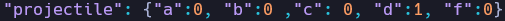
\includegraphics[width=0.6\textwidth]{poly.png}
  \end{center}
  \caption{Json objekt som beskriver en polynom funktion}
  \label{fig:}
\end{figure}
Alla variabler i Json objectet är då konstanterna i polynomfunktionen. Just i figur 1 så beskriver json objektet en projektil som åker snedd längst skärmen. 
Det json objektet beskriver alltså funktionen: 
\begin{figure}[H]
  \begin{center}
    $$y = x$$
  \end{center}
  \caption{Enkel linjär funktion}
  \label{fig:}
\end{figure}
\begin{figure}[H]
  \begin{center}
    $$ ax^4 + bx^3 + cx^2 + dx + f $$
  \end{center}
  \caption{Polynom av fjärde graden}
  \label{fig:}
\end{figure}




\end{document}
